% !TeX program = pdflatex
\documentclass[tikz,border=8pt]{standalone}
\usepackage{pgfplots}
\pgfplotsset{compat=1.16}
\definecolor{FigureBlue}{HTML}{2563EB}
\definecolor{FigureOrange}{HTML}{EA580C}
\definecolor{FigureSlate}{HTML}{475569}
\begin{document}
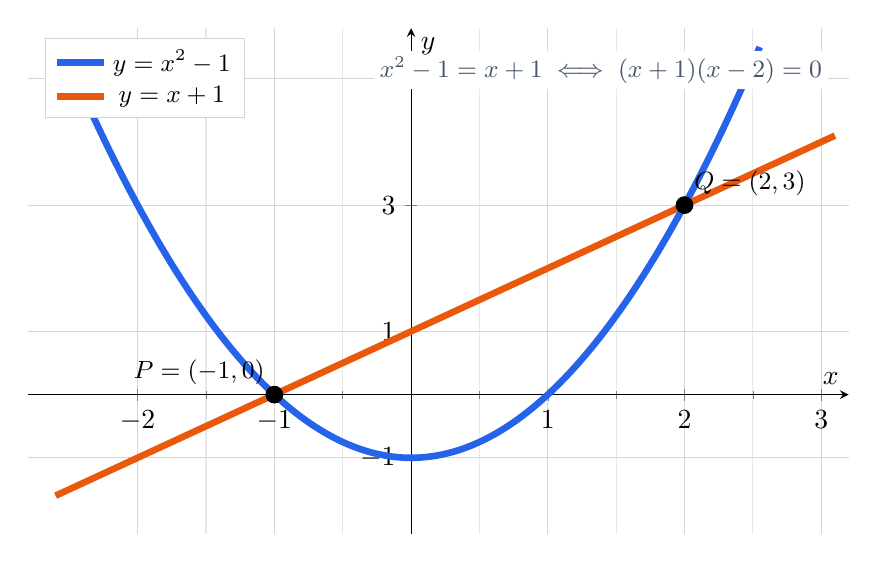
\begin{tikzpicture}
  \begin{axis}[
    width=12cm,height=8cm,axis lines=middle,
    xmin=-2.8,xmax=3.2,ymin=-2.2,ymax=5.8,
    xlabel={$x$},ylabel={$y$},xtick={-2,-1,0,1,2,3},ytick={-1,0,1,3,5},
    grid=both,minor tick num=1,grid style={draw=gray!18},major grid style={draw=gray!32},
    legend style={at={(0.02,0.98)},anchor=north west,draw=gray!35,fill=white,font=\small},clip=false,
  ]
    \addplot[FigureBlue,line width=2.4pt,domain=-2.55:2.55,samples=181] {x^2-1};
    \addlegendentry{$y=x^2-1$}
    \addplot[FigureOrange,line width=2.4pt,domain=-2.6:3.1,samples=2] {x+1};
    \addlegendentry{$y=x+1$}
    \addplot[only marks,mark=*,mark size=3pt,black] coordinates {(-1,0) (2,3)};
    \node[anchor=south east,font=\small] at (axis cs:-1,0) {$P=(-1,0)$};
    \node[anchor=south west,font=\small] at (axis cs:2,3) {$Q=(2,3)$};
    \node[anchor=north east,fill=white,inner sep=2pt,text=FigureSlate,font=\small]
      at (axis cs:3.05,5.45) {$x^2-1=x+1\iff(x+1)(x-2)=0$};
  \end{axis}
\end{tikzpicture}
\end{document}
